\documentclass[a4]{article}
\usepackage{psfig}

\title{De ToolBus}
\author{Pieter Olivier}
\begin{document}
\maketitle

De ToolBus is een software systeem dat software componenten met
elkaar laat samenwerken. 
De ToolBus regelt de communicatie tussen componenten
('tools' geheten in ToolBus terminology),
en zorgt ervoor dat die communicatie zich aan bepaalde regels houdt.
Elk systeem heeft andere regels nodig, en deze regels worden opgeschreven
in een zogenaamd 'ToolBus script'. In dit script schrijft de ontwikkelaar
van een ToolBus systeem precies op welke componenten
met elkaar mogen communiceren. Dit gebeurt door een aantal processen
(zeg maar: kleine programmaatjes) te beschrijven die de communicatie
regelen.

Een ToolBus script wordt geschreven in
een 'formele' taal. Dit wil zeggen dat sommige interessante eigenschappen
van een ToolBus script (en dus van de communicatie tussen de componenten)
met behulp van wiskundige technieken aangetoond kunnen worden.

Belangrijk hierbij is dat \emph{alle} communicatie via de ToolBus
gaat, dus componenten kunnen niet onderling met elkaar praten.
Dit wil dus zeggen dat de ToolBus een zeer centrale rol speelt in
het systeem (Figuur \ref{toolbus}).

\begin{figure}[htb]
\centerline{\psfig{file=arch-simpel.ps,width=6cm}}
\caption{De ToolBus}
\label{toolbus}
\end{figure}

E\'en van de sterkste punten van de ToolBus is dat het programmeertaal
onafhankelijk is. Het maakt niet uit in welke programmeertaal een component
geschreven is, want met behulp van een klein stukje software worden alle
gegevens afkomstig van die component eerst naar een formaat vertaald
dat de ToolBus begrijpt. Op deze manier is het bijvoorbeeld ook mogelijk
om veel bestaande programma's aan de ToolBus te koppelen.

Er zijn al heel wat ToolBus applicaties ontwikkeld om te kijken
of de ToolBus in de praktijk ook nuttig is. Het gaat hier niet alleen om 
`serieuze' applicaties en onderzoeksapplicaties, maar ook om een aantal
leuke spelletjes. Het blijkt namelijk dat het ToolBus concept erg
geschikt is om spelletjes tussen meerdere spelers tegelijkertijd te
beschrijven.

\section*{Zeeslag (Battleships)}

Zeeslag is een leuk spel voor twee partijen, dat een zeeslag simuleert.
Eerst onderhandelen de twee partijen over de grote van het speelveld en
het aantal schepen op het veld. Dan plaatsen ze ieder voor zich de
schepen op hun eigen speelveld, waarna het eigenlijke spel begint. Nu raden
beide spelers om de beurt een positie op het veld van de tegenstander.
Als op de betreffende positie een schip ligt, tekent de computer op 
de betreffende positie een rood hokje, anders een blauw hokje.
Als alle posities die door een bepaald schip bestreken worden geraakt
zijn, is het schip 'gezonken'.

Winnaar is de speler die als eerste alle schepen van zijn tegenstander
gezonken heeft.

Tijdens elke fase van het spelen kunnen beide partijen boodschappen
naar elkaar sturen met behulp van een speciaal invoer veld aan de onderkant
van het zeeslag window.

\begin{figure}[htb]
\centerline{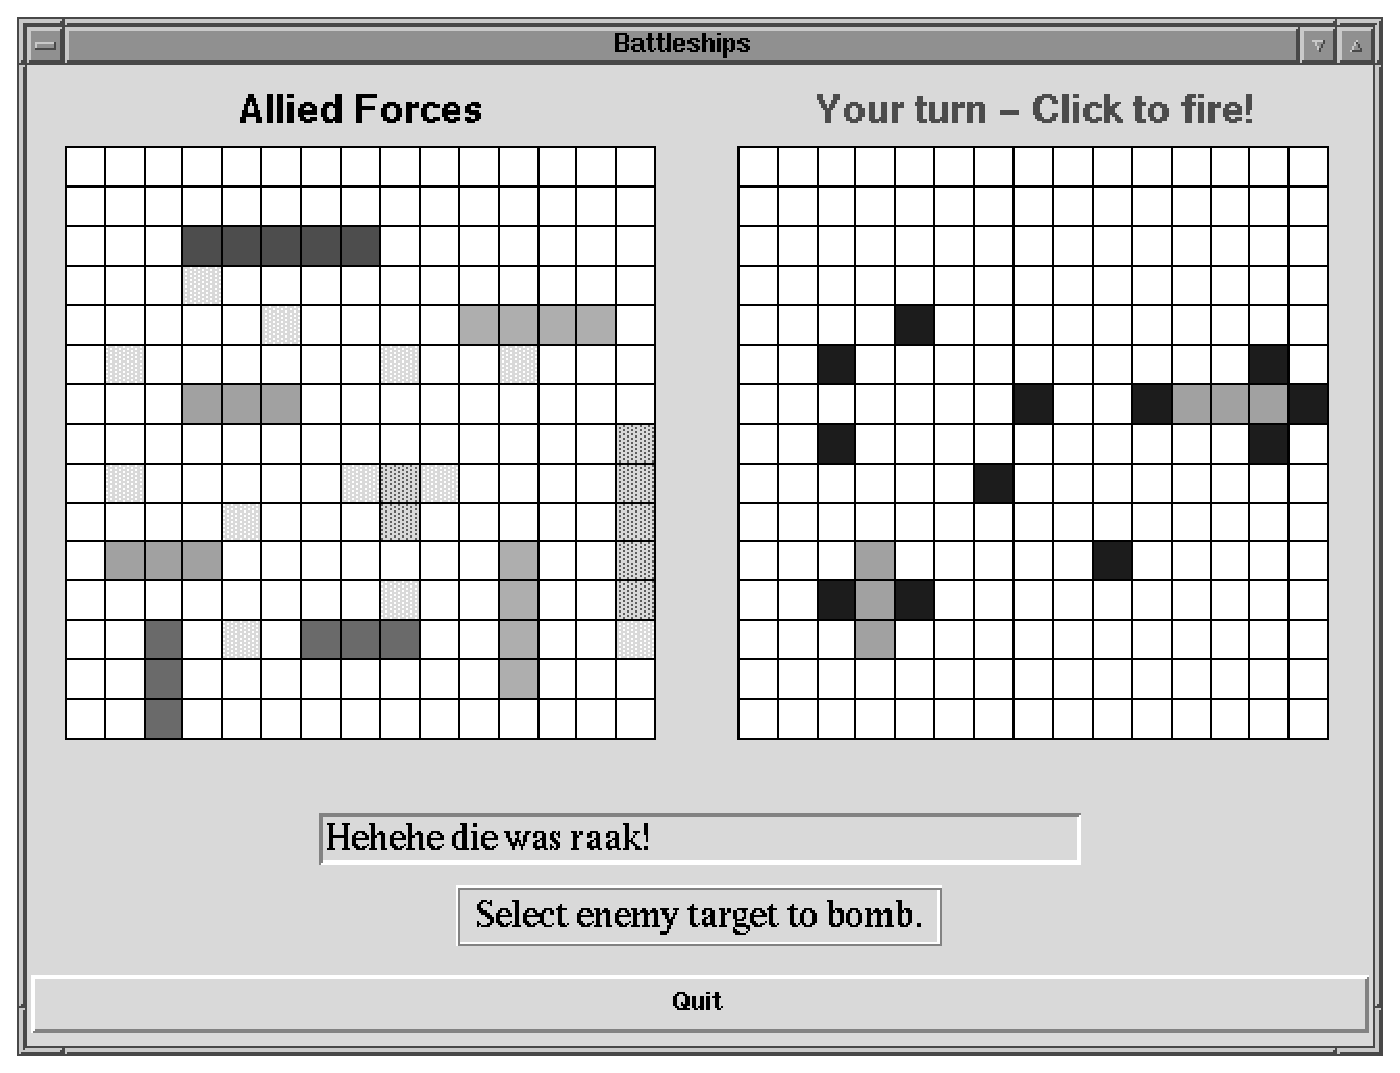
\psfig{file=battleships.eps,width=10cm}}
\caption{Zeeslagje}
\label{battleships}
\end{figure}

Figuur \ref{zeeslag} geeft een overzicht van zeeslag als ToolBus systeem.
Zeeslag bestaat uit drie afzonderlijke componenten die doormiddel van de
ToolBus met elkaar verbonden zijn. Twee van de drie componenten zijn de
programma's die de twee gebruikers op hun scherm krijgen. De derde
component is de scheidsrechter die bekijkt of een schot raak is of niet
en dit aan beide spelers doorgeeft.

\begin{figure}[htb]
\centerline{\psfig{file=zeeslag.ps,width=6cm}}
\caption{Zeeslag als ToolBus systeem}
\label{zeeslag}
\end{figure}


\end{document}
